\section{Modelli di computazione}
Per poter sviluppare un sistema distribuito, è utile definire diversi modelli per l'esecuzione, in modo da poter
classificarli (modelli diversi possono avere vantaggi/svantaggi a seconda del sistema che si deve andare a realizzare).
La maggior parte dei modelli purtroppo sono troppo astratti per poter essere realmente utili da un punto di vista
ingegneristico, cioè non riescono a comprendere in toto la \textit{complessità} reale.

Le prime distinzioni che si possono fare sono su come si possono prendere le decisioni:
\begin{itemize}
 \item modelli \textit{statici}: le decisioni vengono prese prima dell'esecuzione. Risulta quindi essere meno
flessibile, e non si può variare nel corso dell'esecuzione, fornendo quindi poca qualità di servizio.
\item modelli \textit{dinamici}: in questo modello le decisioni risultano essere maggiormente costose, proprio perché
si prendono mentre il modello è in esecuzione.
\end{itemize}
Per fare un esempio, il collegamento fra un client e un Name Server come deve essere stabilito? In maniera statica o
dinamica? E fra il client e server? Si tratta di problematiche da risolvere in fase di progettazione, tenendo conto
dei costi. Un middleware introduce questi costi, fornendo possibilità statiche/dinamiche (non esiste un sistema
totalmente dinamico, realmente totalmente aperto).
Una seconda distinzione riguarda la reazione in caso di errori o concorrenza:
\begin{itemize}
 \item modelli \textit{preventivi}: si fornisce un \textit{comportamento garantito}, oppure si previene/evitano
determinati errori. E quindi un sistema rigido, che presenta dei \textit{costi fissi}.
\item modelli \textit{reattivi}: il modello reagisce in maniera dinamica alle situazioni che si presentano: non è
prevista quindi una \textit{politica di default}, non si stabiliscono risorse a priori come nel caso precedente,
fornendo un comportamento più flessibile. I costi risultano essere variabili, a seconda della complessità del sistema
(al crescere degli attori, aumenta il numero necessario di lock/semafori da utilizzare, per esempio). Il costo può
quindi essere limitato a seconda delle esigenze.
\end{itemize}
\textbf{Esempio:} una serie di clienti vogliono accedere in maniera univoca ad
una risorsa unica: si tratta quindi di un problema
di sincronizzazione e mutua esclusione. Si potrebbe risolvere fornendo dei quanti di tempo decisi a priori per ogni
singolo cliente, oppure si fornisce un token, per cui chi lo possiede è l'unico a poter accedere alla risorsa.

È da osservare che un sistema distribuito in generale offre un insieme di \textit{politiche diverse}, che si possono
mescolare a seconda delle esigenze: un sistema moderno infatti deve essere in grado di seguire l'evoluzione dei servizi
per poter sopravvivere (es CORBA: in versioni successive aggiunge supporto al Web).

Un ulteriore modello semplice da descrivere riguarda in che modo le risorse
sono associate alle applicazioni:
\begin{itemize}
 \item Siamo in \textit{monoutenza} se le risorse sono tutte dedicate all'applicazione descritta
 \item Altrimenti si parla di \textit{multiutenza}: più complessa, ma decisamente più diffusa. Infatti, un numero
superiore di applicazioni può portare ad un uso più efficiente delle risorse.
\end{itemize}
A seguito, si può ragionare quindi come sono disponibili le risorse:
\begin{itemize}
 \item Modello \textit{workstation}: le risorse sono concentrate su un unico nodo.
 \item Modello \textit{processor pool}: le risorse sono distribuite, e vengono associate in maniera trasparente al
servizio.
\end{itemize}

\subsection{Processi o oggetti?}
Un'ulteriore distinzione riguarda su cosa basarsi per descrivere effettivamente come avviene l'esecuzione.
Un primo modello si basa sull'idea del \textit{processo}, che incarna la capacità di esecuzione della macchina. Si
specificano quindi delle operazioni, e si tratta di modelli che tengono conto della macchina su cui si lavora, e
funzionano molto
bene con risorse locali e stato locali. Vi sono più modelli:
\begin{itemize}
 \item \textit{Processi alla Unix}: si tratta di processi pesanti, ognuno dotato
di un proprio stato locale. In questo modello
interessa solo in che modo i processi possono comunicare, essendo lo stato non
condivisibile.
 \item \textit{Processi alla Java}: i processi son leggeri, hanno uno stato
condiviso che può essere usato anche per comunicare.
Risulta essere più facile fare anche dei cambi di contesto, ma si possono
presentare delle interferenze.
\end{itemize}

I thread di una JVM, proprio perché dotati di uno stato condiviso, si possono rapportare con un'altra JVM. I thread
leggeri utilizzano lo stato comune per comunicare.

Un'altra idea riguarda la modellazione basata sul paradigma ad oggetti. È importante ricordarsi che questi son sempre
delle astrazioni, e quindi necessitano di una concretizzazione successiva. Anche qui si possono supporre due diversi
modelli:
\begin{itemize}
 \item \textit{Oggetti passivi}: i classici oggetti alla Java. Rappresentazione l'astrazione di dati su cui delle entità
esterne possono lavorare. Non sono quindi dotati di capacità propria d'esecuzione. Si può quindi avere concorrenza
fra diversi processi che vogliono accedere allo stesso oggetto, non si ha un buon confinamento e si ha scarsa
protezione.
  \item \textit{Oggetti attivi}: sono oggetti dotati di propria
capacitàd'esecuzione. I processi quindi non entrano nell'oggetto, perché vi è
già all'interno dell'oggetto una propria logica di gestione (si ha quindi un
modello a request/response: un processo richiede di poter usare l'oggetto
mediante i ``metodi'' forniti da questo, e questo in base alla sua schedulazione
risponde alla richiesta. È sempre da osservare che un oggetto attivo ha comunque
un proprio stato interno, descritto da una parte sequenziale, ma a cui non vi si
accede con dei metodi, proprio grazie a questa logica interna: i metodi veri e
propri sono utilizzati solo internamente!). Un oggetto attivo è quindi dotato di
una coda delle richieste che si sono presentate, e una sua politica di
scheduling. Si supera in questo modo il problema degli oggetti passivi,
proteggendo del tutto l'oggetto e determinandolo completamente. Un oggetto
attivo quindi, massimizzando la parte sequenziale, si può spostare più
facilmente. Rappresenta lo stesso modello dei servitori paralleli, e, per
esempio, degli agenti mobili. Un oggetto attivo quindi si preoccupa di tutta la
gestione dell'esecuzione internamente (richieste, attività, errori, processi
interni...): si forniscono meccanismi, mediante il quale si possono specificare
delle politiche diverse!
\end{itemize}

Come mai in Java tale modello non è stato implementato? Si tratta di un
\textit{modello molto costoso}, che non presenta delle scorciatoie utili se si
lavorasse solo in ambito locale!
Nei sistemi moderni, in realtà si parla di classi che contengono le definizioni
degli oggetti, e definiscono lo stato interno e i metodi con cui accedere. In
particolare, in generale si parla di semantica per riferimento, che però è in
grado di funzionare solo in un ambito locale. Per riferire in remoto, serve un
supporto esterno. Per esempio, si parla di utilizzare socket, protocolli
standard de facto come TCP/IP...
Tuttavia, è proprio questo il motivo per cui si vengono a definire dei middleware, ovvero delle strutture in grado di
fornire un supporto completo alla comunicazione in remoto. Per esempio, Java Remote Method Invocation è un sistema in
grado di estendere la semantica per riferimento locale, al remoto, cercando di fornire un sistema omogeneo per poter
accedere sia ad oggetti locali che remoti. Nel caso specifico di RMI, per esempio, si utilizza un classico pattern dei
middleware, il \textit{proxy come delegato per la comunicazione}. Si realizzano
infatti uno stub lato cliente e uno skeleton lato
server, che riescono a garantire un qualcosa di simile alla normale comunicazione locale. Si cerca di presentare
un sistema trasparente per l'utente!

Perché quindi non realizzare tutti i riferimenti come riferimenti remoti? È sempre una questione di costo, sarebbe
inaccettabile. Basta pensare a cosa succede ad un oggetto passato via RMI: deve essere serializzabile, e così tutti
i suoi componenti, in maniera che si possa fare marshalling e unmarshalling.
Ciò non è sempre possibile in Java RMI (si pensi ad un oggetto che riferisce un oggetto di tipo File, una risorsa
strettamente locale). Vi sono poi altri problemi da considerare:

\begin{itemize}
 \item Un oggetto remoto viene registrato in un apposito registry, ma se
 viene deattivato? Come viene gestita quindi la persistenza? E lo stato remoto?
 \item Due stub diversi possono riferire lo stesso oggetto remoto? Se sì come si
 gestisce la concorrenza?
 \item Come risolvere i nomi? Si può usare un riferimento fisso, ma l'oggetto
 può essere diverso (ma non è il caso di Java).
 \item Si deve anche passare l'indicatore della classe, perché si possa realmente utilizzare l'oggetto: cosa succede
 se la classe è già presente? Java per esempio controlla mediante l'hash se la classe è effettivamente quella corretta.
\end{itemize}

\subsection{Deployment dell'applicazione}
Un'applicazione distribuita spesso necessita che sia suddivisa in diversi componenti, anche allocati su nodi diversi!
Un componente è un'entità con una granularità superiore all'oggetto, ovvero introduce comportamento e interazione,
estendendo l'idea dell'oggetto.
Se si hanno quindi diversi componenti, che devono dialogare fra di loro, non è detto che il deployment su una singola
macchina sia la soluzione ideale: infatti, su un solo processore si ha una sequenzializzazione delle operazioni, e
quindi dell'applicazione stessa.
Spesso e volentieri, un middleware non si occupa del deployment, ma deve essere realizzato da chi gestisce l'interazione
fra i componenti. L'allocazione può essere statica, cioè decisa prima dell'esecuzione, oppure dinamica, quindi
durante; quest'ultimo modello permette di poter spostare le risorse a seconda delle esigenze durante l'esecuzione.
Spesso e volentieri, l'allocazione viene realizzata utilizzando dei semplici file batch, rendendola semi-manuale (certe
configurazioni devono poi essere sistemate a seconda dei casi dall'operatore).
L'approccio misto è quello più usato, essendo una via di mezzo fra l'allocazione esplicita (tutta a carico dell'utente)
e quella implicita (decisa in toto dal sistema).

\subsection{Altri modelli oltre il C/S}
Esistono diversi altri modelli oltre il classico C/S:
\begin{itemize}
 \item \textit{Push}: il servitore fornisce il servizio al cliente
 \item \textit{Pull}: il cliente recupera il servizio che necessita in maniera diretta.
 \item \textit{Modello a delega}: il cliente delega un altro agente per attendere il risultato, e poi lo recupera da
 questo.
 \item \textit{Modello a notifica}: simile al precedente, solo che il delegato notifica al cliente la disponibilità
 del risultato.
 \item \textit{Modello ad eventi}: il tipico modello consumer/provider, in cui chi è interessato si registra a chi
 produce gli eventi.
 \item \textit{Modello a provisioning}: oltre agli end-point, vi sono intermediari interessati al risultato.
\end{itemize}
Di particolare interesse è la classificazione dei modelli a scambio di messaggi:
\begin{itemize}
 \item In fase di progettazione, si parla di sistemi sincroni se si è interessati al risultati, altrimenti asincroni.
 \item In fase implementativa, si parla di comunicazione bloccante se il richiedente si blocca in attesa del risultato,
 altrimenti non bloccante
\end{itemize}
Oltre alla classicazioni principali, altre caratteristiche con cui si possono classificare i modelli a scambio di
messaggi:
\begin{itemize}
 \item In fase di progettazione si parla di:
 \begin{itemize}
  \item un \textit{sistema simmetrico} se mittente e ricevente si conoscono
  (rarissimo) oppure \textit{asimmetrico} (caso tipico :C/S).
  \item un sistema diretto (cioè se avviene una comunicazione diretta fra i
  processi), oppure indiretto (se si utilizzano strutture tipo le socket)
 \end{itemize}
 \item In fase di implemtazione si parla di:
 \begin{itemize}
  \item un \textit{sistema bufferizzato} se la comunicazione richiede un certo
  numero di messaggi prima di poter trasmettere
  \item \textit{sistemi reliable} se possono fornire QoS, senza perdere
  messaggi.
 \end{itemize}
\end{itemize}
Nel caso si introduca un terzo oggetto che faccia da mediatore, si può quindi lavorare in maniera sincrona ma non
bloccante: è il mediatore che resta in attesa, sganciando il ricevente. Si possono avere due diverse modalità:
\begin{enumerate}
 \item \textit{Oggetti poll}: è un contenitore per la risposta alla richiesta, che viene periodicamente interrogato
 dal ricevente con un sistema a polling. Si ha così una comunicazione a 3 entità. In questo modello, il ricevente
 deve sapere dove si trova l'oggetto poll, e vi deve essere un oggetto per ogni risultato. E conveniente se si hanno
 operazioni corte, e attese brevi.
 \item \textit{Oggetti callback}: è sempre un oggetto che conterrà il risultato, ma dotato di una sua vita
 indipendente, e dotato di codice particolare da eseguire quando giunge il risultato. E lui quindi a dover fornire il
 risultato al richiedente, svincolandolo del tutto da questo! Conveniente in caso di operazioni lunghe, indipendenti
 dal chiamante.
\end{enumerate}
Spesso e volentieri, questi intermediari vengono realizzati da proxy, che sono in grado di ridurre la complessità
logica della soluzione, integrando diverse funzionalità.
In un modello basato sugli eventi, si ha un fortissimo disaccoppiamento (non vuol dire che non si conoscono, ma che
non è necessario che siano attivi contemporaneamente per poter fare la comunicazione; è una caratteristica
fondamentale per i middleware) fra le entità interessate al risultato, e quelle che forniscono i servizi. In questo
modello si ha quindi un'interazione molti a molti, per cui si può facilmente mappare il multicast. In generale gli
eventi non sono persistenti, tuttavia non è l'unico modello possibile.
\subsection{Spazi di tuple}
Un modello che deriva dall'astrazione della memoria condivisa e della comunicazione, e che garantisce il
disaccoppiamento fra le varie entità è lo spazio di tuple. È un meccanismo generale per la comunicazione e la
sincronizzazione, in cui si specifica uno spazio di informazioni fortemente tipato. (Una tipica informazione può essere
\texttt{<mittente, destinatario, data>}, per cui tutti i dati devono essere
diversi perché possa essere inserita).
Si hanno quindi due operazioni principali: la \textit{out} consiste nell'inserire nello spazio delle tuple un nuovo
messaggio, mentre la \textit{in} (bloccante) estrae la prima tupla che fa match
con il criterio indicato (in caso di più tuple che facciano match, è una scelta
non deterministica). Ovviamente, si avrà sempre un numero inferiore di in
rispetto alle out. Se la in è \textit{completamente specificata}
\footnote{specifichiamo l'esatto contenuto della tupla che stiamo cercando}, si
parla di sincronizzazione e non di comunicazione. Uno spazio di tuple permette
anche l'introduzione di QoS, grazie alla persistenza della tupla nello spazio.
Gerlenter, con Linda, presenta due diversi modelli:
\begin{itemize}
 \item \textit{A ring}: si partiziona lo spazio delle tuple, per cui ogni nodo conosce precedente e successivo: si ha
 una conoscenza locale, quindi limitata. Un produttore può fare una out su un qualsiasi nodo, e il messaggio fa un
 ciclo per verificare che non sia già presente su un qualche nodo. Lo stesso discorso vale per la in, che fa un giro
 fino a trovare un messaggio che fa match. In Linda sono state considerate ovviamente delle problematiche di
 replicazione (il messaggio deve essere ripetuto? Ma quindi lo si deve togliere da tutti i nodi che lo contengono),
 sfruttando gli hash dei messaggi
 \item \textit{A matrice}: le out vengono eseguite sulle righe, mentre le in si fanno sulle colonne.
\end{itemize}
\subsection{Modelli a contenimento}
Si tratta di supporti presenti in ogni middleware: sono funzionalità che aggregano diverse attività utili, che si
possono replicare. In questo modo, uno sviluppatore si concentra soltanto sullo sviluppo della business logic vera e
propria, utilizzando le politiche di default fornite dal middleware per quanto riguarda il supporto al tempo di vita,
il gestore della concorrenza, fornire la QoS, sistemi di nomi... Fondamentalmente, un container è un delegato che si
comporta come supervisore di certe attività.
\subsection{Il problema della trasparenza}
Esistono diversi signicati per la trasparenza: per esempio, si intende per l'allocazione l'indipendenza dalla località
delle risorse. In generale, per trasparenza si intende un sistema in grado di fornire all'utente finale un comportamento
omogeneo, anche se ai livelli sottostanti sta lavorando con oggetti/servizi diversi (remoti/locali, server
principale/copia...).
Non è sempre un elemento positivo, perché in molti casi i sistemi son così complessi, che non si possono gestire in
maniera totalmente trasparente: si richiede l'intervento dell'utente. Un esempio è nella trasparenza dell'allocazione:
se non sappiamo dove si trova l'utente, come facciamo a dargli il servizio desiderato? La trasparenza non è corretta
a livello di infrastruttura in questo caso; l'utente infatti è sempre più coinvolto.
Per esempio, TINA-C\footnote{Si tratta di un consorzio di aziende per le telecomunicazioni, con l'obiettivo di andare
oltre OSI: l'idea è quella di immaginare anche i possibili servizi, fornendo un modello più coordinato, e
un'infrastruttura con molti provider: si definisce un accordo/negoziazione fra i fornitori dei servizi e i clienti,
per poter per esempio stabilire la QoS, e quindi si fornisce il servizio con i parametri indicati} prevede sia un
sistema trasparente, che un sistema non trasparente in cui si possano definire le risorse inizialmente, e quindi
introdurre la trasparenza.
\subsection{Le macchine astratte}
Sono stati sviluppati diversi modelli per l'esecuzione, ma alla base vi è la
\textit{Random Access Machine}: è una macchina special purpose, con codice
inalterabile, in grado di eseguire istruzioni in sequenza (tutte le istruzioni
hanno la stessa durata), memoria composta da una sequenza di parole capaci di
contenere un intero e un sistema di input e uno di output.
Un primo modello per la comunicazione è la \textit{Parallel RAM} (PRAM), in cui
si immagina diversi programmi da eseguire contemporaneamente. Una PRAM è
costituita quindi da P macchine RAM, ognuna delle quali esegue un programma, e
ad ogni clock vengono eseguite P istruzioni. Alla base vi è una memoria
condivisa, per tutte le macchine, dove scrivere e leggere i risultati (anche i
dispositivi di I/O sono unici per tutte le macchine). Si tratta di un modello
MIMD (Multiple Instruction Multiple Data) sincrono, per cui quando tutti i
programmi finiscono, anche la macchina termina. Essendo dotata di un'unica
memoria, come devono essere strutturate le operazioni? La concorrenza è un
requisito difficile da realizzare, in confronto al mettere le operazioni in
sequenza. Le diverse PRAM si possono quindi categorizzare a seconda della
tipologia delle operazioni (in generale si hanno letture concorrenti e scritture
sequenziali (CREW - Concurrent Read Exclusive Write); la concorrenza è invece
utilizzata per il sistema di I/O, per limitarne il collo di bottiglia). Un PRAM
è difficile da realizzare perché non è scalabile.
Un secondo modello è il \textit{Message Passing RAM}, che è sempre una
collezione di RAM, ma ognuna con la sua memoria dedicata (i sistemi di I/O son
sempre condivisi). Si ha quindi che le diverse macchine comunicano mediante dei
canali prestabiliti (vi devono essere almeno P-1 connessioni). Si hanno
istruzioni ad hoc, cioè delle send e receive con rendez-vous, una semantica
sincrona: questo vuol dire che un'operazione sblocca la sua duale. Una MP-RAM è
più facilmente realizzabile, e rappresenta meglio un modello locale. Se per
esempio si volesse eseguire un broadcast,
servirebbero almeno P-1 istruzioni, mentre una PRAM, per quanto più difficile
da realizzare, richiederebbe una sola operazione: è un modello con maggiore
capacità espressiva. Restano comunque entrambi dei modelli troppo astratti per
poter essere implementati realmente. Aggiungendo vincoli e limitandoci quindi ad un'ipotesi di località, il progetto
risulta più facilmente realizzabile.
\subsection{Indicatori dell'efficienza}
In generale, ci si limita alla complessità temporale, $T_P(N)$, dove $P$ è il numero di processori considerati: se è
pari ad 1, siamo in un ambiente sequenziale.
Un primo indicatore è lo speed-up, che indica l'incremento di prestazioni se si introducessero P processori:
\begin{equation}
S_P(N) = \frac{T_1(N)}{T_P(N)} > 1
\end{equation}
Tuttavia, bisogna sempre tener presente che non tutti i programmi si possono
parallelizzare: ciò dipende se vi sono troppe dipendenze fra le sotto parti.
Un altro indicatore è l'efficienza nell'uso delle risorse:
\begin{equation}
 E_P(N) = \frac{S_P(N)}{P}
\end{equation}
Ma quindi, ciò corrisponde a dire:
\begin{equation}
 E_P(N) = \frac{T_1(N)}{T_P(N)} \cdot \frac{1}{P}
\end{equation}
Possiamo quindi definire lo speed-up massimo:
\begin{equation}
 max(S_P(N)) = P
\end{equation}
E l'efficienza massima:
\begin{equation}
 max(E_P(N)) = 1
\end{equation}
Sotto queste condizioni si avrebbe che tutti i processori lavorano al massimo, ovvero non abbiamo processori idle che
possono risultare inutili. Questi sono coefficienti statistici, validi per tutto l'algoritmo. Quello che si può
osservare è che la situazione ideale la si avrebbe se lo speed-up dipendesse in maniera lineare dal numero dei
processori. Una soluzione ideale non interessante sarebbe se si distribuisse i compiti ai processi in maniera uguale (un
programma totalmente parallelo!), raccogliendo solo alla fine il risultato. In realtà, i casi più interessanti sono
quelli dove si presentano delle dipendenze, per cui necessariamente vi deve essere una parte sequenziale: questo caso
presenta quindi una comunicazione intrinseca, indipendente dal deployment che si viene a realizzare.
Si possono quindi studiare diversi casi basandosi sui fattori di interesse $N$ e $P$. In particolare, si può definire
come fattore di carico, o loading factor:
\begin{equation}
 L = \frac{N}{P}
\end{equation}
che definisce la complessità come viene suddivisa su ogni nodo. Vi possono essere diversi casi:
\begin{itemize}
 \item \textit{N uguale a P}: su ogni processore viene posta una parte molto semplice del problema. Si dice ipotesi
 di identità.
 \item Dipendenza di N da P
 \item Indipendenza, interessante al crescere di N
\end{itemize}
La legge di Grosh stabilisce che la soluzione migliore risulta essere quella
di lavorare sempre nel concentrato... ma ciò non è sempre possibile! Se per
esempio vi sono risorse limitate? Oppure, oltre un certo valore di N, non si
riesce più a lavorare nel concentrato, e la legge è sicuramente inutile nel caso
di vincoli, tipo la presenza di risorse distribuite.
\begin{figure}[htbp]
 \centering
 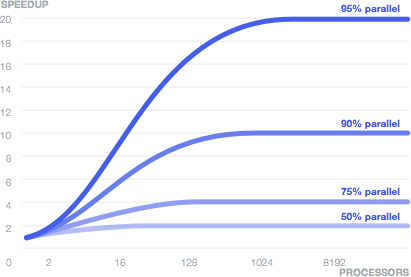
\includegraphics[width=0.8\textwidth]{Images/amdahl.png}
 \caption{Legge di Amdahl [reactivemanifesto.org]}
 \label{fig:amdahl}
\end{figure}
La legge di Amdhal (figura \ref{fig:amdahl}) stabilisce che vi è un limite alla
possibile parallelizzazione, dato che ogni programma è
costituito da una parte parallela e una parte sequenziale, e quest'ultima limita lo speed-up: si ha quindi che non
cresce linearmente, ma tende a un valore asintotico! Nella situazione migliore immaginabile, con le risorse
correttamente allocate, si ha quindi che si avrà uno speedup fisso, mentre sarà l'efficienza a variare a seconda
dell'architettura del sistema!
Come calcolare quindi lo speed-up massimo? Si vuole avere il numero di processori tali che si abbia la minore
complessità del problema, realizzando un sistema fortemente caricato: si definite quindi l'heavily loaded limit:
\begin{equation}
 T_{HL} = \liminf_P{T_P(N)}
\end{equation}
Infatti, si lavora bene caricando molto ogni processore, i quali quindi lavorano per tutto il tempo necessario:
abbiamo quindi in questo modo un buon uso delle risorse.
Tuttavia, per la legge di Amdhal, dobbiamo ricordare che vi è anche una parte sequenziale in ogni programma... che è
proprio la parte di comunicazione fra i diversi processori! Al crescere del numero dei processori, si ha quindi
che lo speed-up diminuisce, allontanandosi dal valore massimo; questo degrado delle prestazioni è dovuto proprio al
peso crescente della comunicazione fra i processori, che diventa fondamentale\footnote{per esempio se la parte
sequenziale è $\frac{1}{5}$ del totale lo speedup massimo sarà il reciproco, ovvero 5}.
\subsection{Caso di studio: somma di N numeri}
Una possibile soluzione, imponendo la condizione d'identità, è quella di utilizzare un albero binario per fare la
sommma: le radici sommano i numeri, che passano il risultato al padre, e così via. Supponendo quindi un albero con
profondità H, possiamo osservare che $N = 2{H+1}$ e $P = 2^{H+1} - 1$, per cui P è simile a N . Si ha che quindi:
\begin{align}
T_P(N) &= O \left(H \right)              \nonumber \\
       &= O \left(\log_2(N)\right)      \nonumber \\
       &= 2 \cdot \log_2 \left(N\right)
\end{align}
Perché 2? Perché abbiamo 2 comunicazioni in ogni nodo. Possiamo quindi valutare l'efficienza di questa architettura:
\begin{equation}
 E_P \left( N \right) = O \left( \frac{1}{log_2\left(N\right)} \right)
\end{equation}
Ma quindi, al crescere di N, l'efficienza tende a 0! Per quanto riguarda lo speedup, si ha che non lavorano tutti i
nodi, ovvero più si risale l'albero e meno i processori lavorano (il processore radice deve attendere, ovvero tempo
di idle, che tutti gli altri abbiano finito!). Se invece avessimo un flusso di dati, i processori risulterebbero
tutti sempre impegnati (potremmo risolvere un insieme di problemi).
Come si possono quindi mantenere sempre impegnati i processori? Si deve incrementare il lavoro sul singolo processore,
per cui:
\begin{equation}
 L = \frac{N}{P} \gg 1
\end{equation}
e quindi la complessità deve essere superiore al numero dei processori: su ogni nodo si ha quindi un certo numero di
valori da sommare. Ciò si può ottenere per esempio con un albero fisso, ovvero un numero di processori fissi. Infatti:
\begin{equation}
 T_P\left(N\right) = O \left(L + \log_2 \left(P\right)\right)
\end{equation}
I due componenti rappresentano rispettivamente il tempo di computazione e quello di comunicazione.
\begin{align}
 S_P(N) &= \frac{T_1(N)}{T_P(N)} \nonumber \\
        &= O \left( \frac{N}{\frac{N}{P} + \log_2(P)} \right) \nonumber \\
        &= O \left( \frac{P}{1} + \frac{P}{N \cdot \log_2(P)} \right)
\end{align}
Per cui, lo speed-up tende effettivamente a P
\begin{align}
 E_P(N) &= \frac{S_P(N)}{P} \nonumber \\
        &= O \left(\frac{1}{1} + \frac{1}{N \cdot \log_2(P)}\right)
\end{align}
E l'efficienza tende ad 1. Quindi, caricando al massimo i processori ed usandoli correttamente, si ottiene speed-up
ed efficienza massimi.
\subsection{Considerare l'I/O}
In questi indicatori si è tuttavia lasciato da parte il problema dell'I/O, che spesso è il vero collo di bottiglia in
diverse architetture. Inoltre, vi son diversi fattori che possono influenzare l'efficienza e lo speed-up
dell'architettura, come il deployment reale. Si possono quindi estendere gli indicatori considerando l'effetto
generale dell'\textit{overhead}, $T_0(N)$, che rappresenta le risorse e il tempo
realmente utilizzato per la comunicazione
(caso ideale di deployment):
\begin{equation}
T_0(N) = \left|T_1(N) - P \cdot T_P(N)\right|
\end{equation}
Ma quindi, si ha che:
\begin{equation}
 T_P(N) = \frac{T_0(N) + T_1(N)}{P}
\end{equation}
E si ha che che lo speed-up risulta essere:
\begin{equation}
 S_P(N) = \frac{P \cdot T_1(N)}{T_0(N) + T_1(N)}
\end{equation}
E che l'efficienza risulta essere:
\begin{equation}
E_P(N) = \frac{1}{1 + \frac{T_0(N)}{T_1(N)}}
\end{equation}
Per cui l'efficienza non sembra dipendere dal numero dei processori... in realtà,
è proprio $T_0(N)$ a dipendere dal numero dei processori: l'overhead dipende dal numero di processori impegnati.
Supponiamo quindi di avere come obiettivo per l'architettura di mantenere costante l'efficienza:
\begin{align}
                            E_P(N) &= \frac{1}{1 + \frac{T_0(N)}{T_1(N)}} \nonumber \\
 E + E \cdot \frac{T_0(N)}{T_1(N)} &= 1                                   \nonumber \\
             \frac{T_0(N)}{T_1(N)} &= \frac{1 - E}{E}                     \nonumber \\
                            T_0(N) &= \frac{1 - E}{E} \cdot T_1(N)        \nonumber \\
                            T_0(N) &= K \cdot T_1(N)
\end{align}
Se K fosse veramente una costante, saremmo in isoefficienza. Un sistema isoefficiente indica che, se manteniamo
costante la complessità e aumentiamo il numero dei processori, l'efficienza non varia. Il valore di K quindi determina
se il sistema ha un buon comportamento. In particolare:
\begin{itemize}
 \item \textit{K piccolo}: il sistema è altamente scalabile. Al crescere di K quindi la scalabilità del sistema decresce
 \item Se non è costante ma funzione dei processori, allora il sistema non è scalabile.
\end{itemize}
I sistemi reali sono scarsamente scalabili.
\subsection{Conclusioni}
Un progetto deve essere valutato attentamente, per cercare di dimensionarlo in maniera corretta: nel caso di una
macchina singola l'heavily loaded limit è un ragionamento corretto, ma bisogna ricordarsi che si deve sempre cercare di
parallelizzare (non utilizzare la legge di Grosh). Per esempio, qual è il numero ideale di processi da realizzare? Si
può ben pensare che avere meno processi di processori risulti in processori che non lavorano, e quindi in un sistema
non efficiente: il limite superiore quindi è che il numero dei processi sia lo stesso del numero dei processori. Un
processore è idle quando comunica, quindi si dovrebbe limitare la comunicazione, e quindi troppi processi comunicano
troppo.
In realtà, statisticamente si ha che un processore che lavora con 20 processi presenta ancora lo stato di idle: un
centinaio di processi per processore è un numero adeguato.
